\section{Introduction}

Ce dossier doit comporter près de dix pages. Il décrit ce comment s’interfacent les composants qui forment le système.

Les questions auquel il répond sont les suivantes:

\begin{itemize}
\item Qui appelle qui et dans quel sens?
\item Quelles sont les informations en entrée?
\item Quelles sont les informations en sortie?
\end{itemize}

Le système a la forme suivante :


\begin{itemize}
\item Production d’énergie

\begin{itemize}
\item Matériel
\item Logiciel

\begin{itemize}
\item Monitoring pile H2
\end{itemize}

\end{itemize}

\item Capteurs

\begin{itemize}
\item Capteurs physiques
\item Module communication

\begin{itemize}
\item Logiciel de relevé des capteurs et de transmission des données
\end{itemize}

\end{itemize}

\item Station

\begin{itemize}
\item Vers capteur

\begin{itemize}
\item Logiciel Réception Stockage données
\end{itemize}

\item Maintenance

\begin{itemize}
\item Interface Logicielle maintenance sur site
\end{itemize}

\item Vers supervision

\begin{itemize}
\item Logiciel traitement ordre Maintenance
\item Logiciel transmission données
\end{itemize}

\end{itemize}

\item Intervention Humaine

\begin{itemize}
\item Réception info technicien

\begin{itemize}
\item Application mobile / Service Web
\end{itemize}

\item Suivi de camions

\begin{itemize}
\item Service Web
\end{itemize}

\item Logistique

\begin{itemize}
\item ERP gestion RH
\end{itemize}

\end{itemize}

\item Supervision

\begin{itemize}
\item Réception

\begin{itemize}
\item Logiciel Réception Stockage Brut
\item Logiciel Transmission Configuration
\end{itemize}

\item Traitement (comprenant Aide à la Décision et Base de Données)

\begin{itemize}
\item Logiciel interprétation
\end{itemize}

\item Restitution

\begin{itemize}
\item Logiciel présentation informations + Services Web
\end{itemize}   
            
\end{itemize}

\end{itemize}


% La figure suivante récapitule ce qui vient d'être dit sous forme de schéma.

\begin{figure}[htb]
\centering
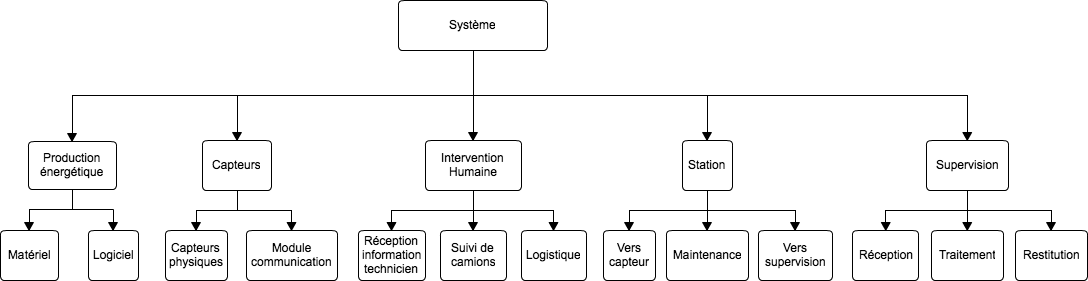
\includegraphics[scale=0.6, angle=90]{system-scheme}
\caption{Schéma de la hiérarchie des composants du système.}
\end{figure}





\section{Production Énergétique}

\subsection{Matériel}

La mise en œuvre d'un module spécialisé pour la gestion de l'énergie n'est utile que pour la détection du niveau d'énergie en réserve. L'interface de ce module s'appuie donc essentiellement sur la mesure du niveau restant.

Les clients de cette interface auront donc pour principale tâche de vérifier à intervalles réguliers le niveau d'énergie en question, pour chaque élément matériel. Ils effectueront donc la requête au module qui gère le matériel correspondant, qui à son tour s'adressera à ce module de production énergétique, dont l'interface est standard.

\begin{itemize}
\item \tt{double getBatteryLevel()}
\item \tt{double precision()}
\end{itemize}

Dans les prochains modules, cette interface sera indiquée comme étant \texttt{struct battery}, structure (ou plutôt classe) que renverront les méthodes de l'interface d'autres modules qui interagissent avec ce module.


\subsection{Logiciel}

La gestion de la production énergétique se fait également au niveau logiciel. L'interface est similaire, mais une problématique supplémentaire vient se rajouter: la partie logicielle étant le composant vital du système, il ne doit jamais être victime d'une panne énergétique.

Il a donc pour but de gérer le niveau d'énergie de la pile à hydrogène, et de lancer une alerte au serveur en cas de besoin, afin qu'une intervention humaine, manuelle, remplace la pile pour maintenir l'intégralité du système en fonctionnement.

Une des conséquences de la vitalité du système est une interface de plus haut-niveau ; tandis que ce comportement est désirable chez les capteurs, qui ont des besoins énergétiques variés, on ne peut laisser à d'autres modules le soin de jauger la criticité du niveau de la pile hydrogène.

\begin{itemize}
\item \tt{enum batteryLevel checkBatteryLevel()}
\item \tt{int sendBatteryLevelAlarm()}
\end{itemize}

Le niveau de la pile possède les champs suivants:

\begin{itemize}
\item \texttt{BATTERY\_FULL} : la batterie a été chargée à bloc.
\item \texttt{BATTERY\_IN\_USE} : la batterie n'est pas pleine, mais elle ne met pas en danger le système.
\item \texttt{BATTERY\_LOW} : la batterie commence à faiblir, il s'agit d'acheter et de prévoir l'acheminement d'une nouvelle batterie hydrogène.
\item \texttt{BATTERY\_CRITIC} : la batterie nécessite un remplacement d'urgence.
\item \texttt{BATTERY\_DEAD} : ce niveau n'est pas sensé être jamais atteint. Il n'existe que pour signaler des dysfonctionnements dans l'approvisionnement d'un site isolé.
\end{itemize}

Ce module pourra être référencé dans les modules suivants comme étant \texttt{struct h2Battery}.


\section{Capteurs}

\subsection{Capteurs physiques}

L'interface des capteurs physiques a pour seul but la lecture de la mesure qu'ils effectuent. Chaque capteur a donc :

\begin{itemize}
\item un numéro d'identification (ou serial number ID), déterminé par le fabriquant,
\item une valeur mesurée (qui peut être obtenue ponctuellement à chaque requête),
\item une valeur représentant le niveau de batterie (qui reste à 100\% si le capteur est câblé).
\end{itemize}

Pour satisfaire cet état des choses, l'interface suivante est mise en place:

\begin{itemize}
\item \tt{string serialID()}
\item \tt{double getMeasure(string serialID)}
\item \tt{string unit(string serialID)}
\item \tt{struct battery getBattery(string serialID)}
\end{itemize}

Il est à noter que la connaissance du niveau de la batterie est acquise non depuis le module "capteur" lui-même, mais depuis le module "production énergétique", avec lequel ce module interagit.

Ce module sera référencé dans les autres modules comme étant \texttt{struct sensor}, une classe qu'utilisent les modules qui interagissent avec les capteurs physiques.


\subsection{Module Communication}

En premier lieu, et conformément au cahier des charges, le module communication s'occupe de l'acquisition et de la transmission des données récupérées par les capteurs.

De ce fait, ce module utilise l'interface des capteurs physiques. Il peut configurer le niveau de batterie considéré comme critique pour chaque capteur. Il peut également détecter l'absence de signal de la part d'un capteur. Cette absence peut être utilisée pour indiquer la mort d'un capteur.

En outre, il est connecté au module de transmission des informations de la station vers le poste de supervision. Il encapsule donc la configuration de la fréquence 

\begin{itemize}
\item \tt{List<struct sensor> getAllMeasures()}
\item \tt{List<struct sensor> getInaccessibleSensors()}
\item \tt{int getBatteryAlarm(string serialID)}
\item \tt{int setBatteryAlarm(string serialID, int level)}
\item \tt{int getTransmissionPeriod()}
\item \tt{int setTransmissionPeriod(int newPeriod)}
\end{itemize}

Ce module sera référencé dans les autres modules comme étant \texttt{struct sensorComm}, une classe qui gère la communication et la configuration des capteurs vis-à-vis de la supervision.


\section{Intervention Humaine}

La question de l'intervention humaine survient lorsque l'on est confronté aux limites de l'automatisation des systèmes que l'on conçoit. En particulier, nous retrouvons la nécessité d'une main humaine au niveau du rechargement des batteries, de la recharge en matière première des sites isolés par camions, de la décharge de produits consommés, ou encore de la réparation des éléments du système trop endommagés pour une réparation à distance.

\subsection{Réception Information Technicien}

Les techniciens ont pour rôle de réparer les dommages physiques exceptionnels qui ne peuvent être effectués à distance, comme dans le cas de la destruction d'un capteur au cours d'une forte tempête. Il doivent également, de façon régulière, remplacer les batteries.

Ce module obtient l'information concernant le bas niveau d'une batterie ou la disparition d'un composant par l'interface proposée par le module communication vu précédemment.

Nous établissons un log de l'état des capteurs et des batteries sur le serveur, afin qu'il soit possible de consulter ces informations.

\begin{itemize}
\item \tt{void logStatus(struct sensorComm commSystem)}
\end{itemize}

Les techniciens peuvent prouver qu'ils ont réparé le système en lançant un simple logStatus, qui mettra à jour les informations concernant la disponibilité de chaque capteur et des batteries.


\subsection{Suivi de camions}

Il s'agit ici de connaître la feuille de route des camions afin de garantir un suivi logistique approprié.

Typiquement, cette interface est utilisée pour enregistrer les mouvements des camions, afin de pouvoir les consulter plus tard sur le site web.

\begin{itemize}
\item \texttt{string getCurrentTarget(string vehicleID)} : obtient le siteID correspondant au site isolé vers lequel le camion \texttt{vehicleID} se dirige, ou \texttt{null}, s'il n'y en a pas actuellement (ou si le véhicule n'existe pas).
\item \texttt{string getPurpose(string vehicleID, string siteID)} : donne le but du voyage identifié par un camion et son objectif.
\item \texttt{struct \{ double latitude, double longitude\} getGeolocalization(string vehicleID)} : récupération des données de géolocalisation envoyées régulièrement par le smartphone du camionneur ou du technicien.
\end{itemize}

Une fois les informations obtenues sur le chargement des camions par communication directe (ie, via le smartphone fourni par COPEVUE) avec les camionneurs, il est possible d'optimiser la logistique à la volée en indiquant au camionneur qu'il peut effectuer un voyage de plus vers un site isolé à proximité, si son camion n'est pas totalement plein, par exemple.

Ces considérations sont mentionnées dans le dossier d'appel d'offre, sans obligation. Notre système permet d'effectuer les optimisations logistiques espérées par effet de bord, et de manière flexible.

\subsection{Logistique}

Tandis que le suivi de camions ne concerne que l'apport de ressources (comme des réserves d'eau, etc.) ou l'embarquement de déchets, la logistique concerne de manière plus générale les flux de ressources qui nécessitent une intervention humaine. Ceci inclut en particulier l'accès à la gestion des routes.

\begin{itemize}
\item \texttt{int addRoute(string vehicleID, string siteID, string purpose)} : ajoute un parcours, indiquant ainsi que le véhicule donné (identifié de manière unique par son vehicleID) se rend au site identifié par siteID. Il est possible d'indiquer la raison du voyage, afin d'offrir des informations supplémentaires à la personne qui consultera par la suite les routes.
\end{itemize}


\section{Supervision}

\subsection{Réception}

\subsection{Traitement}

\subsection{Restitution}

